\chapter{Soluciones de referencia}
\label{cap:capitulo6}

En este capítulo abordaremos una solución de referencia para los ejercicios Sigue-Persona Simulado y Sigue-Persona Real. Con los dos ejercicios el usuario podrá poner a prueba su algoritmo. Se pretende poner en práctica la experiencia del programador robótico cuando desarrolla una aplicación robótica. El primer paso es probar su programa en una simulación (Sigue-Persona Simulado). Una vez que su solución es bastante robusta, pasa al siguiente nivel, probándolo en el mundo real (Sigue-Persona Real). El programador se dará cuenta de que es muy probable que el mismo programa en simulación no funcione exactamente igual con un robot real. Si su solución es bastante buena y robusta, solamente tendrá que ajustar algunos parámetros y tener en cuenta ciertos factores (como por ejemplo la luz ambiental o el rendimiento de CPU) y habrá logrado su objetivo.\\

\section{Solución Sigue-Persona Simulado}
\label{sec:solucion_sigue_personas_simulado}

La solución que resuelve la aplicación de \textit{Seguir a una persona} la podemos dividir en 3 subobjetivos: a) detección mediante redes neuronales y seguimiento mediante un Tracker, b) desarrollo de un algoritmo de evitación de obstáculos y c) creación de una máquina de estados.\\



% -- SUBSECCION TRACKER
% -----------------------
\subsection{Detección mediante RNA y creación de un Tracker}
\label{subsec:ml_tracker}
Para detectar a la persona usamos la función del módulo HAL llamada \textit{getBoundingBoxes}. Esta función realiza una inferencia del modelo de red neuronal para detectar todos los objetos posibles dada una imagen de entrada y devuelve una lista de objetos de cajas de detección (explicados en la Sección [\ref{sec:plantilla_python}]). Crearemos una función llamada \textit{draw\_bounding\_box(img, bbox, color=(23, 230, 210), thickness=2)} con la que podremos dibujar sobre la imagen una caja de detección dada como entrada. En este caso usaremos el color verde (0, 255, 0) e iteraremos sobre todos las cajas de detección obtenidas (Figura \ref{fig:deteccion_ssd_sin_filtro})\\

\begin{figure} [H]
  \begin{center}
    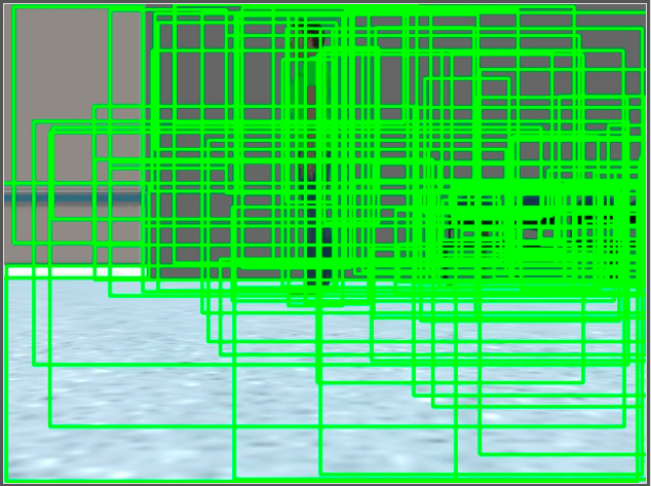
\includegraphics[width=10cm]{imagenes/cap6/deteccion-ssd-sin-filtro.png}
  \end{center}
  \caption[Detección mediante SSD sin filtro]{Detección mediante SSD sin filtro}
  \label{fig:deteccion_ssd_sin_filtro}
\end{figure}\

Un modelo de red neuronal genera una puntuación o \textit{score} para cada objeto detectado dependiendo de su entrenamiento. Por ejemplo, en una imagen donde puede aparecer una persona y una escultura humana, es probable, que la persona detectada tenga una puntuación de un 90 \% y la escultura un 70 \% debido a su parecido. Está en la labor del programador filtrar por \textit{score} para desechar los falsos positivos. Para ello, generamos una función que llamaremos \textit{bounding\_boxes\_by\_score(bounding\_boxes, score\_limit)} que filtre aquellas cajas de detección que superen una puntuación límite. Debido a la naturaleza de este modelo neuronal preentrenado, las óptimas detecciones se han comprobado empíricamente que funcionan con una puntuación superior a 0.3 (el rango va de 0 a 1). Aplicando el filtro obtenemos el siguiente resultado (Figura \ref{fig:deteccion_ssd_filtro_score})\\

\begin{figure} [H]
  \begin{center}
    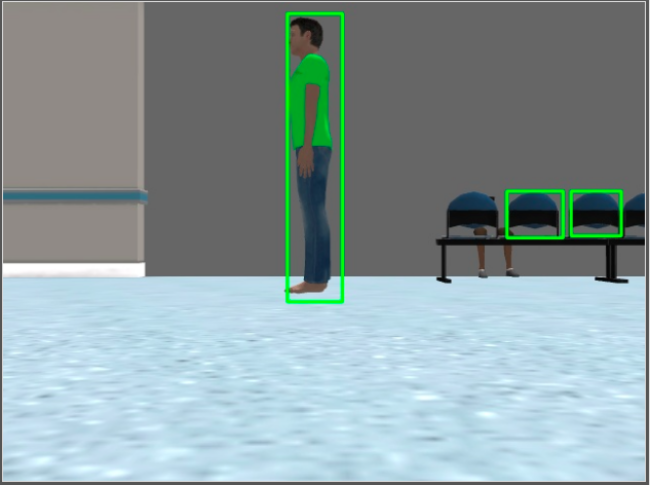
\includegraphics[width=10cm]{imagenes/cap6/deteccion-ssd-filtro-score.png}
  \end{center}
  \caption[Detección mediante SSD filtrando la puntuación de clasificación]{Detección mediante SSD filtrando la puntuación de clasificación}
  \label{fig:deteccion_ssd_filtro_score}
\end{figure}\

Tal y como vemos en la Figura \ref{fig:deteccion_ssd_filtro_score}, tras el filtro de puntuación obtenemos una imagen donde hay tres cajas de detección detectadas: una persona y dos sillas. Para quedarnos solo con las personas aplicaremos un \textit{segundo filtro}, en la cual nos fijaremos en la clase del Bounding Box. Recordemos que el objeto Bounding Box tenía un atributo \textit{id} que correspondía a un número entero y un atributo \textit{class\_id} que era la traducción de dicho número a una cadena de texto (ej: 1 - ``person", 2 - ``bicycle"). Crearemos una función llamada \textit{bounding\_boxes\_by\_name(bounding\_boxes, name)} al cual dada una lista de objetos detectados pasaremos como segundo parámetro de entrada el nombre de la clase que queremos filtrar (en este caso ``person"). Aplicando el filtro obtenemos una correcta detección de personas (Figura \ref{fig:deteccion_ssd_filtro_score_class}):\\

\begin{figure} [H]
  \begin{center}
    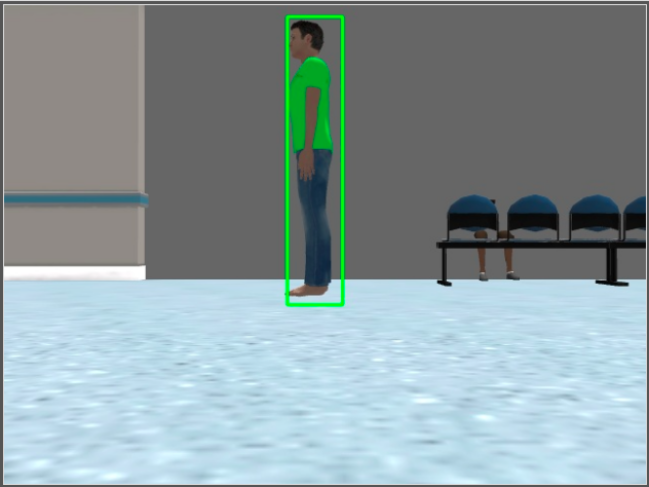
\includegraphics[width=10cm]{imagenes/cap6/deteccion-ssd-filtro-score-class.png}
  \end{center}
  \caption[Detección mediante SSD filtrando la puntuación y la clase]{Detección mediante SSD filtrando la puntuación y la clase}
  \label{fig:deteccion_ssd_filtro_score_class}
\end{figure}

Como último filtro y muy recomendable, debemos rechazar aquellas detecciones que no superen un \textit{área} determinado. Con este filtro, evitamos que el robot se confunda con personas que se encuentren a una distancia lejana o con un falso positivo. Para ello, crearemos una función llamada \textit{bounding\_boxes\_by\_area(bounding\_boxes, min\_area)} al cual dada una lista de objetos detectados pasaremos como segundo parámetro de entrada el área mínimo que debe filtrar.\\

El siguiente paso es crear un \textit{Tracker} de seguimiento. Nuestro \textit{tracker} se basa en la distancia de los centroides de las cajas de detección del fotograma actual con el candidato del fotograma anterior. Recordemos que una caja de detección tenía otros 4 parámetros más: $x_{min}$ e $y_{min}$ correspondían a las coordenadas (x,y) del extremo superior izquierdo de la caja de detección, y $x_{max}$ e $y_{max}$ correspondían a las coordenadas (x,y) del extremo inferior derecho. Para obtener el centroide aplicamos la siguiente fórmula:\\
\begin{eqnarray*}
C_x = \frac{x_{min} + x_{max}}{2}\\
C_y = \frac{y_{min} + y_{max}}{2}\\
\end{eqnarray*}

Creamos una clase llamada \textit{BoundingBoxObject} que tiene 3 atributos: La caja de detección correspondiente, su centroide y su área. El área lo obtenemos de la siguiente manera: $A = (x_{max} - x_{min}) (y_{max} - y_{min})$.\\

Posteriormente, creamos una clase llamada \textit{Tracker} que proporcionará una capa de abstracción al usar los siguientes métodos que definimos:

\begin{itemize}
	\item \textbf{setObjective(self, obj)}: Establece el objetivo BoundingBoxObject de seguimiento.
	\item \textbf{getObjective(self)}: Devuelve el objetivo \textit{BoundingBoxObject} actual de seguimiento.
	\item \textbf{getObjectiveFromSet(self, objlist)}: Dada una lista o conjunto de objetos \textit{BoundingBoxObject}, devuelve el objetivo candidato que más se acerca al anterior, y lo actualiza. El candidato seleccionado será aquel cuyo centroide esté más cerca del actual, no supere una distancia límite(50) con él, y que la diferencia de área entre el \textit{BoundingBoxObject} anterior y el actual sea menor a 30000. Para calcular la distancia entre centroides usaremos la Distancia Euclídea:
	\begin{equation*}
	d = \sqrt{(C_{x}' - C_{x})^2 + (C_{y}' - C_{y})^2}
	\end{equation*}
\end{itemize}\

En la Figura \ref{fig:obtencion_centroide} se puede ver con más detalle en qué se basa este procedimiento: se compara cada centroide con el centroide candidato del fotograma anterior y se elige aquel que cumpla los requisitos descritos anteriormente.\\

\begin{figure} [H]
  \begin{center}
    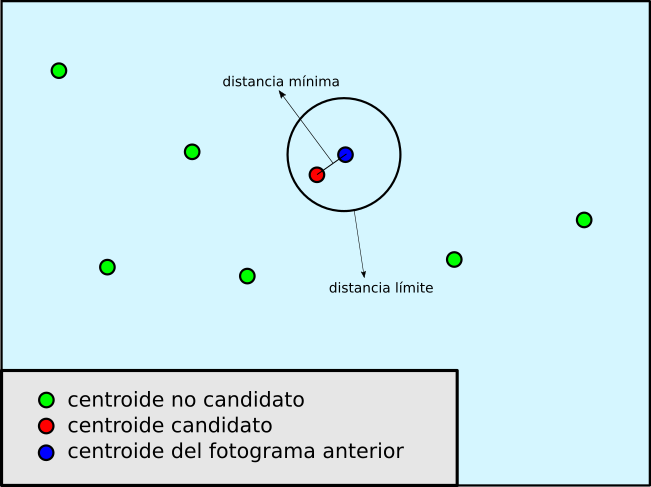
\includegraphics[width=10cm]{imagenes/cap6/esquema-tracker.png}
  \end{center}
  \caption[Modo de obtención del centroide candidato]{Modo de obtención del centroide candidato}
  \label{fig:obtencion_centroide}
\end{figure}\

Al principio del programa inicializamos una instancia de tipo Tracker, y, en cada iteración del bucle principal llamamos al método \textit{getObjectiveFromSet(self, objlist)} para obtener un \textit{BoundingBoxObject} que dibujamos en la imagen de color rojo. El resultado queda de la siguiente manera:\\

\begin{figure} [H]
  \begin{center}
    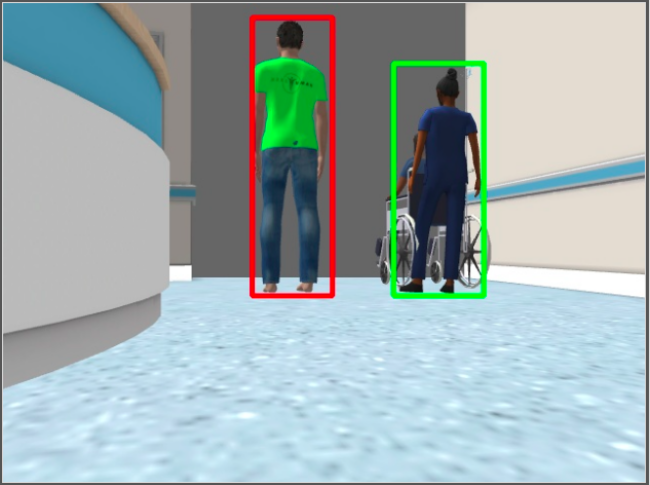
\includegraphics[width=10cm]{imagenes/cap6/aplicando-tracker.png}
  \end{center}
  \caption[Usando el Tracker para no perder al objetivo]{Uso del Tracker para no perder al objetivo}
  \label{fig:uso_tracker}
\end{figure}\

Como criterio de selección de la persona a la que seguiremos, deberá cumplir los 3 filtros indicados anteriormente, aparecer en el segundo tercio de la imagen (dividiremos la imagen en 3 y analizaremos la mitad) y ser aquel \textit{BoundingBoxObject} con un área mayor que el resto.\\


% -- SUBSECCIÓN EVITAR OBSTÁCULOS
% ---------------------------------
\subsection{Algoritmo de navegación VFF}
\label{subsec:vff}

Seguir a una persona en un mundo vacío es sencillo, pero cuando el entorno presenta obstáculos, es importante tener ese riesgo en cuenta:

\begin{itemize}
	\item ¿Qué ocurre si la persona que seguimos gira por un pasillo a la derecha? ¿El robot sufriría una colisión con la pared antes de girar?
	\item ¿Qué ocurre si el robot se está acercando a la pata de una mesa? ¿Y si está pasando cerca de otra persona a la que ha descartado en el proceso de Tracking?
\end{itemize}

El algoritmo de \textit{Campo de Fuerzas Virtuales (VFF)} está muy indicado para esas situaciones. Se basa en la suma vectorial de un vector de atracción y de repulsión originando un vector resultante que indica la nueva dirección de desplazamiento. La suma vectorial estará influenciada por el valor de unos pesos $\alpha$ y $\beta$ aplicados a los vectores de atraccion y repulsión respectivamente, pudiendo de esta manera dar más valor a uno que otro.\\

El \textit{vector de atracción} será aquel que desde el robot apunta al objetivo. Al usar una cámara en la que no tenemos en cuenta la profundidad, establecemos que el módulo del vector será siempre 2 metros. Para obtener el ángulo nos basaremos en el Campo de Visión (FOV) horizontal de la cámara. Al ser una cámara simulada, en su fichero \texttt{camera.urdf.xacro} (tal y como vimos en el capítulo \ref{cap:capitulo4}) indicamos que FOV fuera 1.04 radianes (60 grados). Por lo tanto, 0 grados se corresponderá al centro de la imagen y los extremos a los ángulos -30 y 30. Para conocer el ángulo con el objetivo necesitaremos conocer el ancho de la imagen, y la posición de la coordenada x del centroide. La ecuación es la siguiente:

\begin{equation*}
\alpha = \frac{H_{FOV} \cdot C_{x}}{w} - \frac{H_{FOV}}{2}
\end{equation*}\\

Conociendo el ángulo ($\alpha$) y módulo (m) podremos obtener las componentes x e y del vector de atracción \textit{A}:
\begin{eqnarray*}
A_x = m \cdot sin(\alpha)\\
A_y = m \cdot cos(\alpha)\\
\end{eqnarray*}

El \textit{vector de repulsión} se calculará a partir de todas las lecturas del láser. Cada obstáculo presente en el rango del láser provocará un vector en sentido contrario cuyo módulo estará influenciado por una constante y será inversamente proporcional a la distancia con el obstáculo (es decir, cuanto más cerca, mayor será el módulo). Sabiendo la constante (K) y la distancia (d) de cada lectura del láser (n lecturas), la ecuación del vector de repulsión (R) es la siguiente:

\begin{eqnarray*}
R_x &=& \sum_{i=1}^n\left(\frac{K}{d_i}\right)^2 \cdot cos(\alpha)\\
R_y &=& \sum_{i=1}^n\left(\frac{-K}{d_i}\right)^2 \cdot sin(\alpha)\\
\end{eqnarray*}

En la ecuación vemos cómo la componente $R_y$ va en dirección contraria al desplazamiento del robot. La potencia de 2 se aplica para evitar mínimos locales.\\

El \textit{vector final (F) o resultante} lo obtenemos sumando las componentes de los vectores de atracción y repulsión. Ambos multiplicados por dos constantes $\alpha$ y $\beta$ respectivamente. La ecuación queda de esta manera:

\begin{eqnarray*}
F_x &=& \alpha \cdot A_x + \beta \cdot R_x\\
F_y &=& \alpha \cdot A_y + \beta \cdot R_y\\
\end{eqnarray*}

Queda en la labor del programador ajustar empíricamente los parámetros $\alpha$ y $\beta$ dependiendo del comportamiento que desee. Si queremos darle más peso a la repulsión aumentaremos $\beta$ pero en casos extremos podríamos llegar a perder el objetivo. En cambio, si queremos darle más peso a la atracción conseguiremos que evite los obstáculos sin perder al objetivo pero si está mal ajustado podríamos colisionar a causa de una escasa repulsión. En la Figura \ref{fig:esquema_vff} resumimos el algoritmo VFF de manera gráfica para una mejor comprensión.\\

\begin{figure} [H]
  \begin{center}
    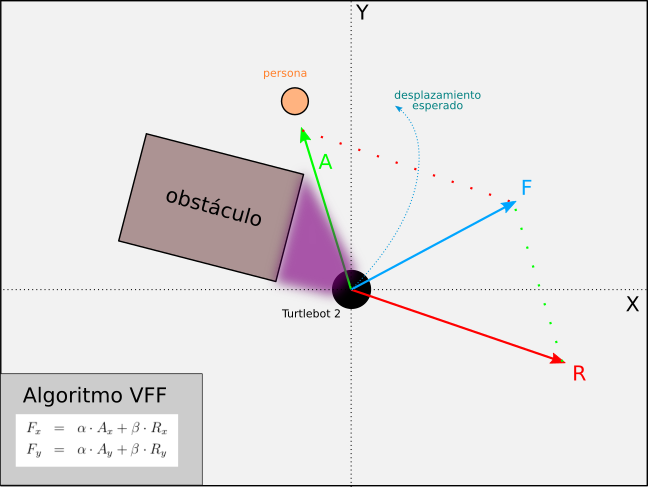
\includegraphics[width=10cm]{imagenes/cap6/esquema-vff.png}
  \end{center}
  \caption[Algoritmo VFF]{Algoritmo VFF}
  \label{fig:esquema_vff}
\end{figure}\

En nuestra solución de referencia, los valores $\alpha$ y $\beta$ que usamos fueron 0.5 y 0.05 respectivamente. Aplicamos solamente la componente $F_x$ del vector final como velocidad angular, ya que la velocidad lineal está \textit{basada en casos} dependiendo de la distancia al objetivo. Esta última depende del tamaño de la caja de detección:

\begin{itemize}
	\item Si el área es menor que 16000, el objetivo se encontrará lejos, por tanto comandaremos una velocidad lineal de 0.2 m/s.
	\item Si el área se encuentra entre 16000 y 45000, significa que el objetivo está cerca, por tanto comandaremos una velocidad lineal de 0.1 m/s.
	\item Si no se cumple ninguna de estas condiciones, el objetivo se encontrará muy cerca por tanto el robot se detendrá.
\end{itemize}\


% -- SUBSECCION MÁQUINA DE ESTADOS
% ----------------------------------
\subsection{Máquina de Estados}
\label{subsec:maquina_estados}

Como último paso de la solución, queda implementar una máquina de estados que le dé al robot la capacidad de tomar distintas acciones dependiendo del estado en el que se encuentre. En nuestro caso, hemos definido 2 estados: Buscar-Persona y Seguir-Persona.\\

El estado \textit{Buscar-Persona} será aquel con el que empecemos la ejecución del programa. Al principio, girará a una velocidad angular determinada mientras aplica los 3 filtros de detección sobre la imagen para detectar personas. Transitará al siguiente estado cuando el robot identifique un candidato a seguir (mayor área del \textit{BoundingBoxObject} y posicionado en la franja central de la imagen).\\

En el estado \textit{Seguir-Persona} aplicaremos el algoritmo de \textit{Tracking} y VFF. Además, la velocidad lineal cambiará dependiendo de la distancia al objetivo. Para ello crearemos unas condiciones en las que dependiendo del área de la caja de detección aplicaremos una velocidad u otra. Cuanto más pequeño sea el área, más lejos estará nuestro objetivo. Si por algún motivo perdemos a la persona, incrementaremos un contador de fallo y de esta manera, en caso de no detectarla en el siguiente fotograma, nos quedaremos con el mismo valor del centroide candidato. Cuando el contador supere un límite, transitaremos al primer estado: \textit{Buscar-Persona}.\\

En la Figura \ref{fig:maquina_estados} se puede ver un esquema de la Máquina de Estados Finitos (FSM) utilizada.\\

\begin{figure} [H]
  \begin{center}
    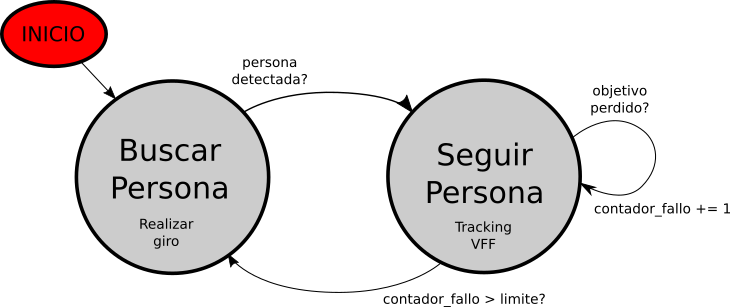
\includegraphics[width=12cm]{imagenes/cap6/maquina-estados.png}
  \end{center}
  \caption[Máquina de Estados Sigue-Persona]{Máquina de Estados Sigue-Persona}
  \label{fig:maquina_estados}
\end{figure}\


\subsection{Validación experimental}
\label{subsec:validacion_experimental_sim}

A continuación describiremos la ejecución de la solución de referencia donde pusimos en prueba nuestro algoritmo:

\begin{itemize}
	\item Para probar el algoritmo de navegación VFF, colocamos dos objetos de Gazebo en frente del robot con el fin de que pudiera esquivarlos sin perder al objetivo. Primero, el robot se encontraba en el estado Buscar-Persona hasta que detecta a su objetivo en el medio de la imagen. Al transitar de estado, el robot comienza a utilizar la navegación VFF con una velocidad lineal de 0.1 m/s debido a la distancia que le separa con la persona. Al principio, debido a la repulsión del obstáculo que tiene a su derecha, el robot gira a la izquierda, pero debido al valor incremental de la componente $A_{x}$ de la fuerza del vector de atracción, el robot bordea el obstáculo. Seguidamente, realiza lo mismo con el obstáculo que tiene a su izquierda. En la Figura \ref{fig:sim_solucion_vff_test} se puede ver la prueba realizada. Después de esquivar los dos obstáculos, el robot recuperaba su estabilidad.
	
	\begin{figure} [H]
		\begin{center}
		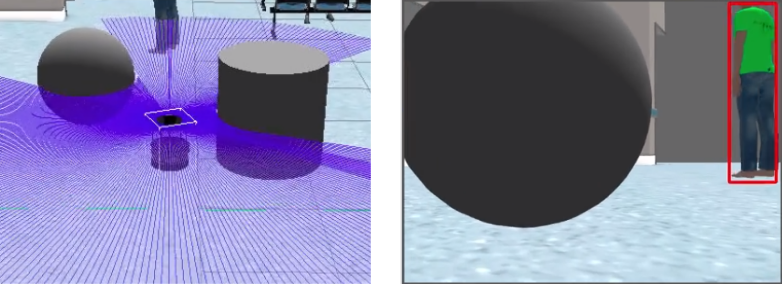
\includegraphics[width=10cm]{imagenes/cap6/sim-solution-vff-test.png}
		\end{center}
		\caption[Solución Sigue-Persona Simulado: prueba de navegación VFF]{Solución Sigue-Persona Simulado: prueba de navegación VFF}
		\label{fig:sim_solucion_vff_test}
	\end{figure}

	\item Luego, para probar el algoritmo de seguimiento (\textit{tracking}), dirigimos a la persona simulada a través del recibidor del hospital (la zona del escenario donde hay más personas) pudiendo comprobar que el robot era capaz de seguir a su objetivo sin confundirse. Poco después de comenzar el seguimiento, utilizamos a la persona simulada para alejarla lo máximo posible del robot y vimos como su velocidad lineal cambiaba de 0.1 m/s a 0.2 m/s. Luego pasamos cerca de una enfermera cuya caja de detección aumentaba en la parte derecha de la imagen conforme el robot se acercaba, pero no perdía a su objetivo inicial. En la Figura \ref{fig:sim_solucion_tracking_test} se puede ver la prueba que realizamos para el algoritmo de \textit{tracking} perceptivo.

	\begin{figure} [H]
		\begin{center}
		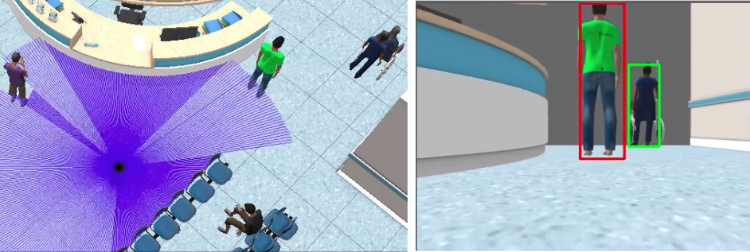
\includegraphics[width=10cm]{imagenes/cap6/sim-solution-tracking-test.png}
		\end{center}
		\caption[Solución Sigue-Persona Simulado: prueba de seguimiento]{Solución Sigue-Persona Simulado: prueba de seguimiento}
		\label{fig:sim_solucion_tracking_test}
	\end{figure}
\end{itemize}\

El vídeo de la solución que muestra todas las pruebas descritas se puede ver en el siguiente enlace: \url{https://youtu.be/fDAU465eVxQ}\\




% -- SECCION SIGUE PERSONAS REAL
% -----------------------------
\section{Solución Sigue-Personas Real}
\label{sec:solucion_sigue_personas_real}

El modo de resolver este problema es idéntico al Sigue-Personas simulado, sin embargo, el entorno sobre el que se mueve el robot, y el rendimiento del ejercicio debido a una distinta carga computacional causada por la ausencia del simulador puede provocar que el comportamiento de la ejecución no sea el esperado.\\

\subsection{Adaptaciones}
\label{subsec:adaptaciones}

En la solución de referencia seguimos los mismos pasos que en la sección \ref{sec:solucion_sigue_personas_simulado} y en algunos de ellos ha sido necesario adaptar o reajustar alguna parte:\\

\begin{itemize}
	\item Implementación del \textit{Tracker} de seguimiento. Los pasos son los mismos:
	\begin{enumerate}
		\item Localizar a una persona aplicando los filtros de \textit{score} o puntuación, clase y área.
		\item Aplicamos el criterio de \textit{selección}: dividir la imagen en 3 secciones y elegir como objetivo la persona más cercana que esté situada en la sección central
		\item Crear una clase Tracker que guarde constantemente y vaya actualizando el objetivo de seguimiento en cada fotograma.
		\item Para no perder al objetivo, en cada fotograma nos quedaremos con el centroide de la caja de detección más cercana al centroide candidato del fotograma anterior, mientras no supere un límite de distancia. En caso de no detectar al objetivo, iremos incrementando un contador de fallo.
	\end{enumerate}
	\begin{figure} [H]
		\begin{center}
			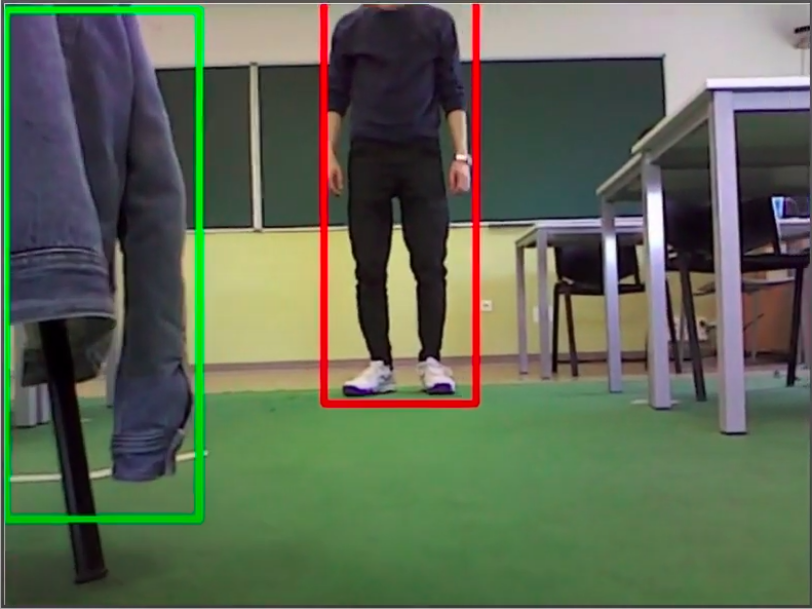
\includegraphics[width=10cm]{imagenes/cap6/tracker.png}
		\end{center}
		\caption[Tracker en el ejercicio Sigue-Persona Real]{Tracker en el ejercicio Sigue-Persona Real}
		\label{fig:tracker_real_follow_person}
	\end{figure}\
	
	\item Implementación del algoritmo VFF. Como la frecuencia de actualización cambia ante la ausencia del simulador, ha sido necesario reajustar los parámetros $\alpha$ y $\beta$ del algoritmo para equilibrar la relación entre la fuerza de atracción y de repulsión. Es recomendable que el párametro $\alpha$ que multiplica a la fuerza de atracción sea mayor que $\beta$ para no perder al objetivo. Sin embargo, tenemos que tener en cuenta que $\beta$ debe estar correctamente ajustado para esquivar con seguridad y suavidad los obstáculos que se encuentre por su camino. Un buen ajuste de parametros permitirá por ejemplo seguir a una persona a través de un pasillo manteniendo la misma distancia con ambas paredes sin importar la colocación de su objetivo. En nuestro caso, los valores de $\alpha$ y $\beta$, comprobados empíricamente, fueron 1.5 y 0.5 respectivamente.
	
	\item Máquina de Estados Finitos. Seguimos usando dos estados maestros: Buscar-Persona y Seguir-Persona. La transición del estado Seguir-Persona a Buscar-Persona estaba determinado por el contador de fallo que indiciamos en el proceso de seguimiento del Tracking. El límite del contador dependerá de los fotogramas por segundo. En el ejercicio Sigue-Persona Simulado, la velocidad de fotogramas era baja por lo tanto el límite era menor, pero en este caso, al haber aumentado la velocidad de refresco, tiene sentido aumentar el límite del contador para que, si perdemos a la persona en un fotograma, podamos seguir guardando el centroide de la última caja de detección candidata.
\end{itemize}\




\subsection{Validación experimental}
\label{subsec:validacion_experimental_real}

Para su validación se realizaron las mismas pruebas que en el ejercicio Sigue-Persona Simulado:\\

\begin{itemize}
	\item Para probar el algoritmo de navegación VFF, pusimos una silla en mitad del escenario (Figura \ref{fig:real_solucion_vff_test} izquierda). Cuando el robot detectaba a su objetivo, empezaba a acercarse, rodeando el obstáculo que tenía a su izquierda. Cada vez que el centroide de la caja de detección se alejaba más del centro de la imagen, mayor era la fuerza de atracción aplicada a la velocidad angular del robot. También, aprovechando el escenario de la \textit{Robocup} en el Laboratorio de Robótica, probamos la navegación a través de un pasillo pudiendo observar que, debido al ajuste correcto de los parámetros de repulsión y atracción, el robot era capaz de seguir a la persona manteniendo la misma distancia con las paredes (Figura \ref{fig:real_solucion_vff_test} - derecha). Una vez que el robot tenía hueco para salir del pasillo, conseguía mantenerse en frente de su objetivo.
	
	\begin{figure} [H]
		\begin{center}
		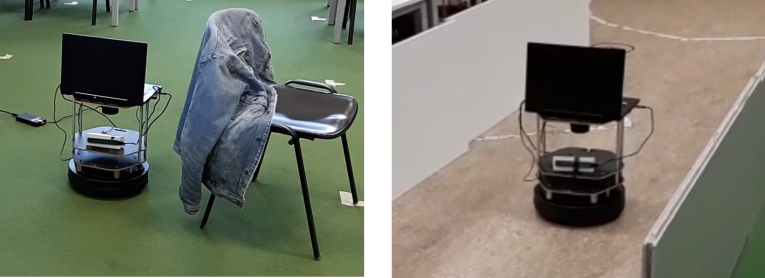
\includegraphics[width=10cm]{imagenes/cap6/real-solucion-vff-test.png}
		\end{center}
		\caption[Solución Sigue-Persona Real: prueba de navegación VFF]{Solución Sigue-Persona Real: prueba de navegación VFF}
		\label{fig:real_solucion_vff_test}
	\end{figure}
	
	\item Durante una de las ejecuciones, después de que el robot detectara a la persona, y la empezara a seguir por el laboratorio, vimos que la detección mostraba un falso positivo en el robot Pepper debido a su aspecto físico parecido al ser humano, además de la chaqueta colocada sobre la silla (Figura \ref{fig:real_solucion_tracking_test}). Como aplicamos el criterio de selección del centroide más cercano al anterior mediante la distancia Euclidea, el robot logra realizar su tarea de seguimiento correctamente.
	
	\begin{figure} [H]
		\begin{center}
		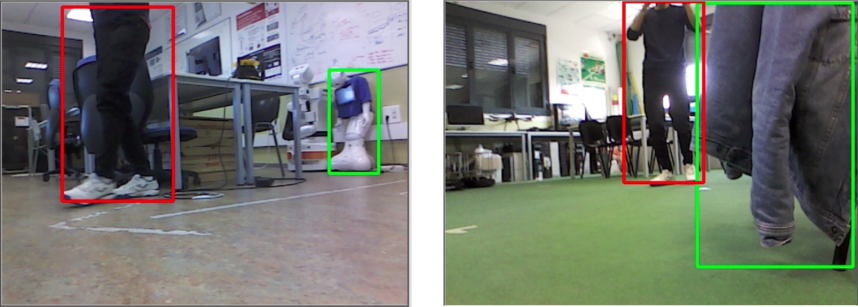
\includegraphics[width=10cm]{imagenes/cap6/real-solucion-tracking-test.png}
		\end{center}
		\caption[Solución Sigue-Persona Real: prueba de seguimiento]{Solución Sigue-Persona Real: prueba de seguimiento}
		\label{fig:real_solucion_tracking_test}
	\end{figure}
\end{itemize}\

El vídeo probando el algoritmo de navegación VFF a través de un pasillo se puede ver a través de este enlace: \url{https://www.youtube.com/watch?v=qIcsjsmKjH8}\\

El vídeo de la ejecución donde mostramos las pruebas descritas esta accesible desde el enlace: \url{https://youtu.be/54Jb4KJwyDM}\\



% -- SECCION VARIANTES
% ----------------------
\section{Variantes alternativas}
\label{sec:variantes_solucion}

La solución mostrada en las secciones \ref{sec:solucion_sigue_personas_simulado} y \ref{sec:solucion_sigue_personas_real} no es lá unica para abordar la aplicación. Podemos enfocar el problema Sigue-Persona de varias maneras. A continuación indicamos algunas posibles opciones que tuvimos en cuenta antes de llegar a la solución final de referencia:\\

\begin{itemize}
	\item \textbf{Control de velocidad basado en franjas}. En este modelo de seguimiento, dividimos la imagen en franjas y dependiendo de la posición $C_{x}$ del centroide usamos una velocidad angular determinada. En el código \ref{cod:vel_bar} podemos ver un ejemplo de implementación.
\begin{code}[H]
\begin{lstlisting}
vels = [0.3, 0.2, 0.1, 0, -0.1, -0.2, -0.3]	 # vel > 0 === left turn

width = img.shape[1]
step = width/len(vels)

while True:
	# ...
	cx, cy = centroid
	# ...
	
	HAL.setW(vels[int(cx/step)]) # Angular velocity
\end{lstlisting}
\caption{Ejemplo de control de velocidad basado en franjas}
\label{cod:vel_bar}
\end{code}
	Esta fue la primera solución alternativa utilizada, cuyo video se puede ver a través de este enlace: \url{https://www.youtube.com/watch?v=58ckb5fFvrs}\\
	La ventaja de este algoritmo es que el movimiento angular está controlado en un rango elegido por el programador y los cambios de velocidad se realizan de manera suave. La desventaja es que puede provocar pequeñas oscilaciones cuando la caja de detección de la persona se encuentre en el centro de la imagen. Además, hay que tener en cuenta la repulsión del láser, cuya suma puede afectar al movimiento del robot al no existir un vector de atracción.
	
	\item \textbf{Velocidad basada en un controlador PID}. Con un controlador PID bien configurado obtendríamos una respuesta rápida y precisa para no perder a la persona. Su algoritmo de seguimiento sería semejante al ejercicio \textit{Follow Line}\footnote{\textbf{Follow Line}: \url{http://jderobot.github.io/RoboticsAcademy/exercises/AutonomousCars/follow_line/}}. Una desventaja de usar un controlador PID es el hecho de verse afectado a causa de una baja velocidad de fotogramas por segundo provocando oscilaciones constantes. Esta alternativa no podría tener en cuenta los obstáculos ya que cuanto más repulsión tuviera el láser, mayor sería la fuerza del controlador PID debido a la acumulación del error.
	
	\item \textbf{Detección de color}. Como solución de escape en caso de tener problemas de alto de rendimiento, pensamos la opción de seguir a la persona dependiendo del color de la camiseta. En el caso del hospital pusimos la camiseta del modelo teleoperado de color verde para facilitar la detección. En un escenario real, la persona podría ponerse alguna camiseta de algún color llamativo para facilitar la detección. Para abordar esa solución, tendríamos que seguir estos pasos:
	\begin{enumerate}
		\item Cambiar el espacio de color de la imagen de RGB a HSV\footnote{\textbf{HSV}: \url{https://es.wikipedia.org/wiki/Modelo_de_color_HSV}}. El espacio HSV (Hue, Saturation, Value) facilita la detección de colores.
		\item Obtener el rango HSV de valores mínimo y máximo del color de la camiseta y crear una máscara que la filtre correctamente.
		\item Siendo $p_{i}$ el valor del pixel (0 o 1) de la máscara y $x_i$ las coordenadas del pixel correspondiente, el centroide lo obtendremos de la siguiente manera (ecuacion obtenida de \cite{centroide_ecuacion}):
		\begin{equation*}
		c = \frac{\sum_{i=1}^n\left(p_i \cdot x_i\right)}{\sum_{i=1}^n\left(p_i\right)}
		\end{equation*}
		\item Una vez obtenido el centroide, aplicar el algoritmo VFF igual que en la solución de referencia.
	\end{enumerate}\
	
	En la Figura \ref{fig:color_deteccion} se puede ver un filtro de color verde que utilizamos al principio para el ejercicio Sigue-Persona Simulado:\\
	
\begin{figure} [H]
	\begin{center}
	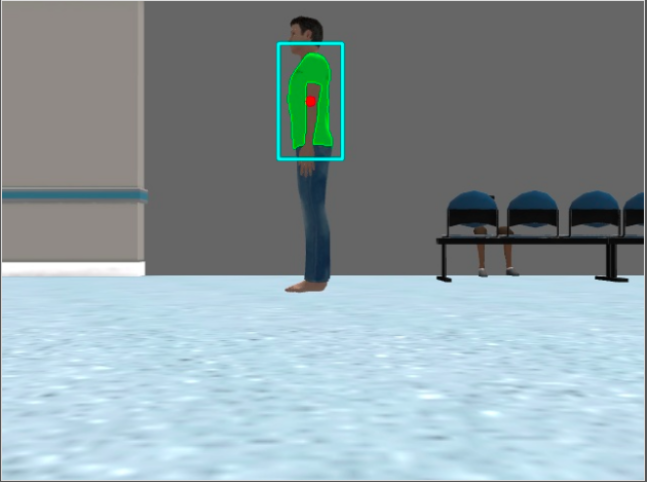
\includegraphics[width=10cm]{imagenes/cap6/deteccion-color.png}
	\end{center}
	\caption[Variante alternativa usando un filtro de color]{Variante alternativa usando un filtro de color}
	\label{fig:color_deteccion}
\end{figure}
	
	La desventaja de esta solución es que la percepción visual basada en filtros de color es frágil porque requiere que la persona a seguir se vista de una determinada manera. Es preferible una percepción basada en RNA porque es mucho más robusta, funciona en un amplio abanico de situaciones y no require que la persona se vista de ninguna manera especial.
\end{itemize}

